\documentclass{article}
\setlength{\parskip}{5pt} % esp. entre parrafos
\setlength{\parindent}{5pt} % esp. al inicio de un parrafo
\usepackage{amsmath} % mates
\usepackage[sort&compress,numbers]{natbib} % referencias
\usepackage{url} % que las URLs se vean lindos
\usepackage[top=10mm,left=20mm,right=20mm,bottom=25mm]{geometry} % \textbf{\textbf{}}margenes
\usepackage{hyperref} % ligas de URLs
\usepackage{graphicx} % poner figuras
\usepackage[spanish]{babel} % otros idiomas

\title{TAREA \#0} %titulo
\author{Natalia Berenice P\'{e}rez L\'{o}pez} % author
\date{\today}

\begin{document} % inicia contenido

\maketitle % cabecera

\begin{abstract} % resumen
  Pr\'{a}ctica sencilla sobre el uso b\'{a}sico de \LaTeX{} en Overleaf.
\end{abstract}
\section{Introducci\'{o}n}\label{intro} % seccion y etiqueta
Esta pr\'{a}ctica es un ejemplo de c\'{o}mo realizar los reportes de nuestras tareas. Incluimos una ecuaci\'{o}n \eqref{equ}:

\begin{equation}
  f(x) = 10 \tanh(x) - \int_0^\infty \frac{5}{10 + x} \text{d}x.
  \label{equ}
\end{equation}

Tambi\'{e}n podemos citar fuentes \citep{ejemplo} \citep{otroejemplo}. Al final se incluye la figura de una flor \ref{flor}.

\begin{figure} % figura
    \centering
    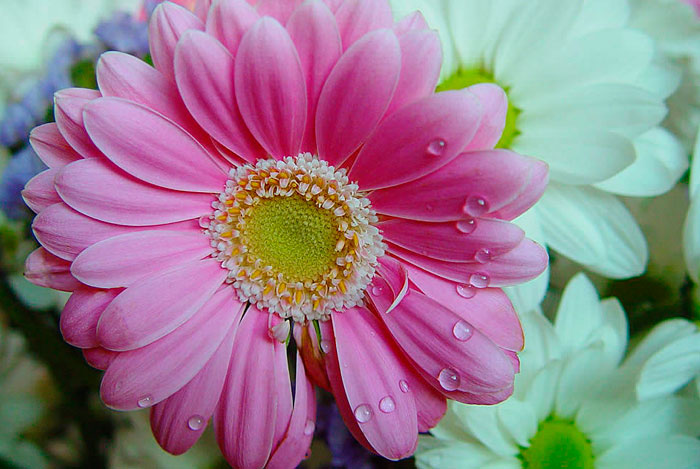
\includegraphics[width=80mm]{flor.jpg} % archivo
    \caption{Flor recuperada de \url{https://www.floresyplantas.net/flores-de-margaritas/} con licencia CC.}
    \label{flor}
\end{figure}

\section{Conclusi\'{o}n}
Realizar este documento me sirvi\'{o} como pr\'{a}ctica para aprender a trabajar en Overleaf.

\bibliography{referencias}
\bibliographystyle{plainnat}

\end{document}